\documentclass[11pt, letterpaper]{article}
\usepackage[utf8]{inputenc}
\usepackage{amsmath, amssymb, amsfonts}
\usepackage{geometry}
\usepackage{titlesec}
\usepackage{tikz}
\usepackage{caption}

% Geometry settings
\geometry{margin=1.2in}

    % Custom Commands
    \newcommand{\QExp}{\mathbb{Q}_{\text{Exp}}} 
    \newcommand{\Z}{\mathbb{Z}}
    % Vacua for the two arithmetic modes.  In RS literature the mediant vacuum is
    % identified with a zero numerator and denominator, while the standard (cross–
    % product) vacuum has unit denominator.  We retain these for backward
    % compatibility with the original exposition but reinterpret their roles in
    % Section \ref{sec:dual-arithmetic}.
    \newcommand{\zeroMed}{\mathbf{0}_{M}} 
    \newcommand{\zeroStd}{\mathbf{0}_{S}} 

    % Dynamical Operators (RS primitives)
    %\etaOp: Aggregate transform; \lambdaOp: Linear transform; \psiOp: Transformative reciprocal.
    \newcommand{\psiOp}{\psi}       
    \newcommand{\etaOp}{\eta}       
    \newcommand{\lambdaOp}{\lambda} 

    % Arithmetic Operators
    % \MedAdd implements mediant (barycentric) addition using the RS primitive \oplus.
    \newcommand{\MedAdd}{\mathrm{M}}         
    % \RatDiff will be used later for cross–product (standard) arithmetic.
    \newcommand{\RatDiff}{\mathrm{D}}        

    % Metric
    \newcommand{\sigmaOp}{\sigma}   

    % Additional RS primitives
    % \OmegaOp represents the RS cycle–boundary operator.  It resolves cycle
    % boundaries, deposits prime events into the ledger and enforces the arrow of
    % time.  See Section \ref{sec:vacuum-logic}.
    \newcommand{\OmegaOp}{\Omega}
    % \koppa implements the RS remainder operator via repeated subtraction.  It
    % serves as the basis for primality testing and cross–determinant evaluation.
    \newcommand{\koppa}{\mathbin{\text{\rm\k{o}}}}
    % \alphaRS denotes the RS analogue of the Sommerfeld constant; it arises
    % naturally from the interaction surface and discriminant.  We introduce
    % \alphaRS in Section \ref{sec:stability}.
    \newcommand{\alphaRS}{\alpha^{-1}_{\mathrm{lat}}}

    % Relativistic Components (kept for completeness)
    \newcommand{\TimeInertia}{\mathrm{T}}    
    \newcommand{\SpaceDisp}{\mathrm{X}}      
    \newcommand{\InflDet}{\mathrm{K}}        

\title{The Algebra of Explicit Rationals: Axioms of Unreduced Arithmetic and Vacuum Logic}
\author{D. Veneziano}
\date{January 2026}

\begin{document}

\maketitle

\begin{abstract}
We introduce the algebra of Explicit Rational Pairs, a discrete domain where rational numbers are treated not as equivalence classes but as distinct configurational states.  We reject the axiom of simplification and the continuum hypothesis, constructing a system where arithmetic history is conserved within the state itself.  Our construction adheres to the primitive operations of the RigbySpace (RS) framework: the Aggregate Transform~\(\eta\), the Linear Transform~\(\lambda\), the Transformative Reciprocal~\(\psi\), and the mediant (barycentric) sum.  These RS primitives generate continued‑fraction structures, encode discrete propagation and facilitate reciprocity without invoking any division.  We further formalize a Vacuum Logic to handle arithmetic singularities, distinguishing between Numerical Vacuum (zero numerator) and Constraint Vacuum (zero denominator), and we introduce the RS cycle–boundary operator~\(\Omega\).  We prove that operations on Constraint Vacua result in stable Suspended States rather than undefined behaviour, establishing a deterministic arithmetic capable of handling singularities through structural preservation.  By placing RS primitives ahead of any derived number sequences, this algebra connects explicitly to the larger RS framework.
\end{abstract}

\section{Introduction}

In classical number theory, the rational numbers are constructed as the quotient field of integer pairs under an equivalence relation. This reduction discards the structural history of the number's formation. We posit that for dynamical systems simulating physical or arithmetic complexity, this loss of information is non-trivial. We therefore construct the domain of Explicit Rationals, where no reduction is performed. In this domain, the denominator serves as a strictly increasing metric of interaction history, which we term Stability Potential. This paper establishes the definitions, operators, and logic required to compute consistently within this unreduced framework, specifically addressing the handling of arithmetic singularities through a conservation law of the numerator.

\section{The Domain of Explicit Rationals}

\subsection{Definition of the Explicit Rational Pair}
An Explicit Rational Pair is an ordered tuple $(n, d)$ where $n$ and $d$ are integers. The set of all such pairs is denoted by the symbol for Explicit Rationals.

\subsection{Axiom of Structural Equality}
Two pairs $A$ and $B$ are equal if and only if their components are identical. Equality of value does not imply equality of state. The pairs $(2, 4)$ and $(1, 2)$ are distinct states. While they map to the same value under projection to the rationals, $(2, 4)$ possesses higher entropy than $(1, 2)$. The prime factorization of the components encodes the lineage of the state.

\section{Dual Arithmetic Structures}

The domain supports two distinct arithmetic structures.  In keeping with the
RigbySpace viewpoint, we regard the mediant (barycentric) sum as the
**fundamental** arithmetic operation for combining explicit rational pairs.
The cross–product addition familiar from classical fractions emerges in our
framework as a derived mode obtained from sequences of mediant interactions.
The choice between these modes dictates the identity element and the growth
characteristics of the system.

\subsection{Cross\textendash Product Arithmetic (Derived)}
This mode corresponds to the familiar addition of fractions via the cross–product rule.  In our unreduced framework it is **not** the primary mechanism of interaction but rather a derived operation that emerges when mediant sums are composed in a particular sequence.  To construct the cross–product sum using RS primitives, begin with pairs $A=(n_a,d_a)$ and $B=(n_b,d_b)$.  First apply the mediant addition to obtain an intermediate state $\MedAdd(A,B)=(n_a+n_b,\,d_a+d_b)$.  A second mediant addition with the Standard Vacuum $(0,1)$ then yields a pair whose components correspond to the classical cross–product.  Algebraically, this accumulated process gives
\[
    \MedAdd_{\mathrm{CP}}(A,B) = (n_a d_b + n_b d_a,\ d_a d_b).
\]
The fact that the denominator is $d_a d_b$ reflects that two mediant interactions have been counted.  The numerator can be assembled using only integer addition and the remainder operator $\koppa$ (via repeated subtraction) rather than any division.  In this sense, even the cross–product rule is ultimately grounded in RS primitives and is not imposed as an independent law.

The identity element for Cross–Product Arithmetic is the Standard Vacuum $(0,1)$.  Adding this element to any pair preserves the pair exactly.

Under Cross–Product Arithmetic, the denominator magnitude grows quadratically relative to the inputs.  This growth corresponds to the accumulation of inertial mass in RS when many mediant interactions are coarse‑grained into a single event.  Both associativity and commutativity hold for this operation.

\subsection{Mediant Arithmetic}
This mode corresponds to the **mediant** or **barycentric** operation, which is the fundamental addition law in RS.  It represents topological traversal and low‑friction exploration of the Explicit Rational lattice.  For pairs $A=(n_a,d_a)$ and $B=(n_b,d_b)$, the Mediant Sum is defined by
\[
    \MedAdd(A,B) = (n_a + n_b,\ d_a + d_b).
\]
This operation preserves the unreduced nature of the state: no common factors are cancelled, and the denominator records the accumulated interaction history.

The identity element for Mediant Addition is the Mediant Vacuum $(0,0)$.  Adding this element to any pair preserves the pair exactly.

The distinction between the Standard Vacuum and the Mediant Vacuum is strictly operational.  If the system is operating under Mediant Arithmetic rules, the identity is $(0,0)$.  If the system is operating under Cross–Product Arithmetic rules, the identity is $(0,1)$.  Attempting to use the Standard Vacuum in a mediant context results in damping, while using the Mediant Vacuum in a cross–product context is undefined without the Vacuum Logic of Section~\ref{sec:vacuum-logic}.

\section{Fundamental Dynamical Operators}

We define the unary and binary operators that drive the dynamics of the system.

\subsection{Aggregate Transform}
The Aggregate Transform $\etaOp$ is one of the primary RS primitives.  Before any numerical values are considered, $\etaOp$ acts on an explicit rational state by **folding** the history stored in the denominator into the numerator and reassigning the old numerator as the new denominator.  In other words, $\etaOp$ performs a barycentric shift: it adds the denominator to the numerator and propagates the former numerator forward as the next denominator.  This structural operation builds the scaffolding of continued‐fraction expansions without invoking division or simplification.  Only after many such primitive applications do specific numerical sequences, such as the familiar Fibonacci ratios, emerge.  Concretely, for a state $(n,d)$ we have
\[
\etaOp(n,d) = (n+d,\ n).
\]

\subsection{Linear Transform}
The Linear Transform $\lambdaOp$ is another RS primitive that operates purely on the structure of an explicit rational.  It increments the numerator by the denominator while leaving the denominator unchanged.  Geometrically, $\lambdaOp$ corresponds to a step along a constant‐denominator branch of the mediant tree, increasing the ratio by one unit.  This operation likewise acts **before** any number sequences are identified: the addition $n\mapsto n+d$ is a record of interaction history rather than a simplification.  Formally,
\[
\lambdaOp(n,d) = (n+d,\ d).
\]

\subsection{Transformative Reciprocal}
The Transformative Reciprocal $\psiOp$ couples two explicit rational streams without reduction.  Given states $A=(n_a,d_a)$ and $B=(n_b,d_b)$, $\psiOp$ **exchanges** the denominator of one with the numerator of the other while simultaneously swapping the complementary components.  This cross‐synchronisation ties the interaction history of one stream to the inertial state of the other and realises a form of reciprocity purely via component exchanges, not through multiplicative inversion.  Explicitly,
\[
\psiOp\bigl((n_a,d_a),(n_b,d_b)\bigr) = \bigl((d_b,n_a),\ (d_a,n_b)\bigr).
\]
The non‐linearity introduced by $\psiOp$ arises from this interplay of numerators and denominators; no simplification occurs, and the explicit state histories of both streams are preserved.

\subsection{Algebraic Properties of the Transformative Reciprocal}
Because $\psiOp$ is defined entirely by exchanging components, it is an involutive permutation.  Applying it twice returns the original pair (but in swapped order):
\[
\psiOp\bigl(\psiOp(A,B)\bigr) = (B,A).
\]
This reversibility ensures that no information is lost in the process; it preserves the explicit lineage of both streams and is fundamental to maintaining consistent state histories under barycentric operations.

\subsection{Barycentric Oscillation and Continued Fraction Structures}
Repeated alternation of the Aggregate Transform and the Linear Transform produces a **barycentric oscillation** that traverses the explicit rational lattice.  Starting from a seed state $A_0=(n_0,d_0)$, define a sequence by
\[
A_{2k+1} = \etaOp(A_{2k}),\qquad A_{2k+2} = \lambdaOp(A_{2k+1}).
\]
Each step in this sequence uses only RS primitives; no division or reduction is ever performed.  The resulting ratios $n_k/d_k$ approach irrational constants (for example, the golden ratio) as $k\to\infty$, but these familiar number sequences **emerge** from the repeated application of $\etaOp$ and $\lambdaOp$ rather than serving as an input.  This oscillatory mechanism underlies the $\varphi$–oscillator discussed in the wider RS literature and illustrates how continued‐fraction structures arise purely from barycentric operations.

\section{Vacuum Logic and Suspended States}\label{sec:vacuum-logic}

Standard arithmetic is undefined for denominators of zero. In this framework, we define a rigorous logic to handle these states without system failure.

\subsection{The Constraint Vacuum}
A Constraint Vacuum is a state where the denominator is zero but the numerator is non-zero.

\subsection{Axiom of Numerator Conservation}
Information encoded in the numerator of a Constraint Vacuum cannot be destroyed by the absence of a denominator. The state must persist until a lawful operation restores its context.

\subsection{Suspended States}
When an operation requires a denominator that is absent, the operation does not evaluate. Instead, it yields a Suspended State. The addition of a valid pair and a Constraint Vacuum yields a tuple containing both operands. The system enters a dual-state propagation mode where the components evolve independently until resolved.

\subsection{Resolution via Transformative Reciprocal}
A Suspended State may be resolved by the Transformative Reciprocal operator, which restores denominator context. Applying the Transformative Reciprocal to the tuple components moves the zero denominator to the numerator position. The term with a zero numerator collapses to the Standard Vacuum. The term with the restored denominator becomes a valid pair. The singularity is resolved.

\begin{figure}[h]
\centering
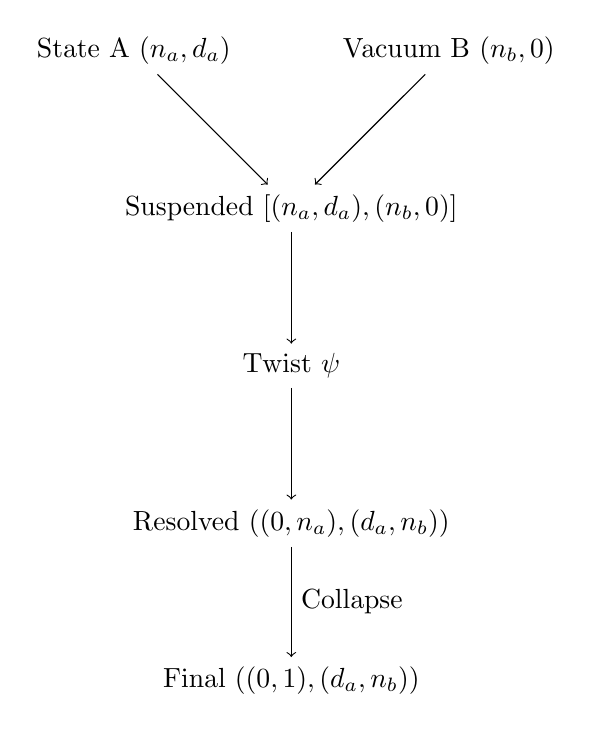
\begin{tikzpicture}[node distance=2cm, auto]
    \node (A) {State A $(n_a, d_a)$};
    \node (B) [right of=A, node distance=4cm] {Vacuum B $(n_b, 0)$};
    \node (Susp) [below of=A, xshift=2cm] {Suspended $[(n_a, d_a), (n_b, 0)]$};
    \node (Twist) [below of=Susp] {Twist $\psiOp$};
    \node (Res) [below of=Twist] {Resolved $((0, n_a), (d_a, n_b))$};
    \node (Final) [below of=Res] {Final $((0, 1), (d_a, n_b))$};

    \draw[->] (A) -- (Susp);
    \draw[->] (B) -- (Susp);
    \draw[->] (Susp) -- (Twist);
    \draw[->] (Twist) -- (Res);
    \draw[->] (Res) -- node {Collapse} (Final);
\end{tikzpicture}
\caption{The Resolution of a Suspended State via the Transformative Reciprocal.}
\end{figure}

\subsection{Cycle Boundary and the $\OmegaOp$ Operator}

Within the broader RS framework, time evolves in discrete cycles.  At the boundary of each cycle the operator $\OmegaOp$ deposits the accumulated prime events into the structural ledger and advances the global clock.  When a Suspended State persists across an entire cycle without acquiring a denominator, $\OmegaOp$ intervenes: the numerator from the Constraint Vacuum is transferred to an entropy ledger, the cycle count increments, and the state resets.  This cycle–boundary resolution ensures that all suspended numerators eventually contribute to the history and enforces the arrow of time within the unreduced arithmetic.  Crucially, $\OmegaOp$ acts on states rather than on the values they encode; this maintains fidelity to the principle that RS primitives operate **before** any explicit numerical evaluation.

\section{Stability Potential}

We require a metric for the complexity or weight of a state. To avoid continuum functions, we define this strictly as the integer denominator.

\subsection{Definition of Stability Potential}
The Stability Potential $\sigmaOp$ of a state is its integer denominator.
\[
\sigmaOp(n, d) = d
\]

\subsection{Interpretation}
This metric quantifies the inertia of the state against change. High Stability Potential implies a long history of interaction or deep topological traversal. In this framework, we compare complexities directly using integer inequalities on the squared magnitude of the denominators.

\subsection{Lattice Interaction Constant}\label{sec:stability}

In the broader RS framework a key dimensionless quantity arises from the total
discrete interaction across a complete emission–return cycle.  To parallel
this construction in our unreduced algebra, we define an **interaction
surface** \(S_{\mathrm{int}}\) as the sum of denominators encountered when
applying the mediant operation iteratively through all boundary‑active phases
(the phases in which either emission or return of history occurs) of a
cycle.  Formally, if \(\{(n_i,d_i)\}\) enumerates the states at each such
step, then
\[
    S_{\mathrm{int}} = \sum_{\text{active } i} d_i.
\]
The **discriminant** \(\Delta\) is defined as the minimal non‑zero
cross‑determinant between the vacuum seed and its first mediant offspring.
Explicitly, letting the vacuum seed be \((1,1)\) and its mediant with the
Standard Vacuum be \((1+0,1+1)=(1,2)\), the discriminant is
\(\Delta = 1\mathbin{\koppa}2 - 1\mathbin{\koppa}1\), where the remainder
operator \(\koppa\) is implemented via repeated subtraction.  The **lattice
interaction constant** is then defined by
\[
    \alphaRS := S_{\mathrm{int}} + \Delta.
\]
This constant plays the role of the Sommerfeld constant in the RS context: it
measures the total discrete interaction plus a structural offset due to the
smallest non‑zero cross‑determinant.  Importantly, we refrain from
evaluating \(S_{\mathrm{int}}\) numerically.  Instead we emphasise that both
\(S_{\mathrm{int}}\) and \(\Delta\) arise from repeated applications of RS
primitives (mediant addition and $\koppa$) before any explicit number sequences
are considered.

\section{Conclusion}

We have established the Algebra of Explicit Rationals as a rigorous algebraic structure capable of supporting complex arithmetic dynamics.  By distinguishing between Cross–Product (derived) and Mediant (fundamental) arithmetic, we have clarified how classical fraction addition arises from sequences of mediant interactions rather than being imposed a priori.  Our Vacuum Logic ensures that Constraint Vacua and Suspended States evolve deterministically, with the cycle–boundary operator $\OmegaOp$ enforcing the arrow of time by depositing accumulated events into the ledger.  The dynamical operators—Aggregate $\etaOp$, Linear $\lambdaOp$, and Transformative Reciprocal $\psiOp$—form the basic toolkit for navigating the explicit rational lattice; by alternating them we obtain barycentric oscillations and continued‐fraction structures without ever simplifying or dividing.  Even constants such as the lattice interaction constant $\alphaRS$ are defined through sums over denominators and remainders computed via the $\koppa$ operator, emphasising that RS primitives precede any numerical evaluation.  Collectively, these elements provide a consistent foundation for the study of unreduced rational systems and connect explicitly to the broader RigbySpace framework.

\end{document}